\documentclass[usenatbib]{mnras}
% for guidance, see phd_work/mnras_guide.pdf
\setlength\parindent{0pt}

\usepackage[english]{babel}
\usepackage[utf8x]{inputenc}
\usepackage[T1]{fontenc}

\usepackage{graphicx}
\usepackage{braket}
\usepackage{amsmath}
\usepackage{multirow}
%\usepackage{natbib}

\begin{document}

\begin{abstract}
The abstract of the paper.
\end{abstract}

\section{Introduction}
\subsection{Motivation}
The fundamental parameters of stars, such as their effective temperatures and metallicities, dictate their observed apparent properties, such as their luminosities and spectra. Hence, a full accounting of the effects of these parameters, and any physical stellar processes that impact on them, directly or indirectly, must be sought.

\subsection{Thermohaline mixing}
The first months of the project were dedicated to the study of thermohaline mixing. This effect was proposed by ****Ulrich (1972) and ****Kippenhahn et al. (1982) to explain anomalous chemical abundances at the surface of mature (i.e post-first-dredge-up), ****low-mass red giant branch (RGB) stars. Specifically, the anomalies consist of an over-abundance of $^{12}$C, $^{16}$O and $^{14}$N, together with a paucity of $^{7}$Li and $^{1}$H, in the stellar spectra. Taken together, these particular changes in these particular species indicate an interaction between the RGB star's fusion shell and the surface, i.e. a mixing effect.

The basic structure of low-mass (< ***Msun) RGB stars, starting from the physical centre of the star, can be summarised as follows:

\begin{enumerate}
\item Inert, electron-degenerate $^{4}$He-dominated core (98$\%$ by mass), generally extending out to a coordinate fractional mass of ~0.28$M_{\star}$.
\item Fusion shell, in which the fusion reactions which previously occurred in the main-sequence core occur now in the RGB phase. The main reactions are the pp-chain and CNO cycle.
\item Radiative zone, consisting of layers for which the Schwartzschild criterion for instability $\nabla _{\textnormal{rad}} > \nabla _{\textnormal{ad}}$ is NOT fulfilled, thus ensuring stability against convection. ****mass For a solar mass RGB star, this extends out to ~0.29***$M_{\star}$
\item Convective zone, where the Schwartzschild criterion is fulfilled, and mixing is modelled using the mixing-length theory (MLT)
\item Atmosphere
\end{enumerate} 

$^{3}\textnormal{He}$ + $^{3}\textnormal{He} \longrightarrow$ $^{4}\textnormal{He}$ + $2^{1}\textnormal{H}$

\begin{equation}
\frac{\partial X_{i}}{\partial t} = \frac{1}{\rho r^{2}}\frac{\partial}{\partial r} \left( \rho r^{2} D_{\textnormal{thl}} \frac{\partial X_{i}}{\partial r} \right)
\label{diffusion_eq}
\end{equation}

\begin{equation}
D_{\textnormal{thl}} = C_{\textnormal{thl}} K \left( \frac{\phi}{\delta} \right) \frac{\nabla _{\mu}}{\nabla _{\textnormal{rad}} - \nabla _{\textnormal{ad}}}
\label{Dthl_def}
\end{equation}

\begin{equation}
K = \frac{4acT^{3}}{3\kappa\rho ^{2}c_{P}}
\label{diffusivity_def}
\end{equation}

\begin{equation}
X_{i,n} = X_{i,n-1} + \delta t \left( \frac{\partial X_{i}}{\partial t}\right)
\label{iter_timeind}
\end{equation}

\begin{equation}
\nabla _{\mu} = \frac{d\ln\mu}{d\ln P}
\label{del_mu_def}
\end{equation}


$\nabla _{\textnormal{ad}} = \left(\partial\ln T / \partial\ln P \right)_{\textnormal{ad}}$

$\nabla _{\textnormal{rad}} = \left(\partial\ln T / \partial\ln P \right)_{\textnormal{rad}}$

\begin{equation}
\mu = \frac{1}{\sum_{i=1}^{i=N} (Z_{i}+1) \frac{X_{i}}{A_{i}}}
\label{mol_weight_def}
\end{equation}



\subsection{Differential extinction}
Extinction of light between a source object, such as a star, and a remote observer is subject to various quantities, such as the density and metallicity of the interstellar medium along the emission travel path.

Bolometric corrections

After accounting for a general extinction effect on an object's emission, its apparent magnitude in a given filter $X$ (i.e. wavelength range, which we define as increasing from $\lambda _{1}$ to $\lambda _{2}$) is given by:

\begin{equation}
m_{X} = -2.5 \log_{10} \left(\frac{ \int_{\lambda_{1}}^{\lambda_{2}} f_{\lambda} \left( 10^{-0.4 A_{\lambda}} \right) S_{\lambda} d\lambda }{ \int_{\lambda_{1}}^{\lambda_{2}} f_{\lambda}^{0} S_{\lambda} d\lambda }\right) + m_{X}^{0}
\label{app_mag_def}
\end{equation}

where $f_{\lambda}$ represents the monochromatic flux at a given wavelength $\lambda$ at the observer distance, $A_{\lambda}$ is the extinction value as a function of wavelength, $S_{\lambda}$ is the response function and $f_{\lambda}^{0}$ and $m_{X}^{0}$ represent the monochromatic flux and apparent magnitude, respectively, of a known reference object in $X$. In this project,the star Vega was used as the reference.

Since our goal, ultimately, is to document potential effects of fundamental stellar properties upon observables, we need to connect the observational and idealised scenarios, for which we use bolometric corrections. For a filter $X$, the extinction parameter $A$ must be ****calibrated relative to a known value. For this reference, in this work we will input a value of the extinction in the well-studied Johnson-$V$ filter.
To derive the equation linking a bolometric correction with the extinction parameter, we start with the definition of a bolometric correction in $X$, $BC_{X}$:

\begin{equation}
BC_{X} \equiv M_{\textnormal{bol}} - M_{X}
\label{BC_def}
\end{equation}

where $M_{X}$ is the absolute magnitude of the object in $X$ and $M_{\textnormal{bol}}$ is its (predicted) absolute bolometric magnitude, defined relative to the Sun using:

\begin{equation}
M_{\textnormal{bol}} = M_{\textnormal{bol},\sun} - 2.5 \log_{10} \left( \frac{4\pi R^{2}F_{\textnormal{bol}}}{L_{\sun}} \right)
\label{mbol_sun}
\end{equation}

where  $F_{\textnormal{bol}}$ is the bolometric stellar flux at its surface, $R$ is the stellar radius, $M_{\textnormal{bol},\sun}$ is the solar absolute bolometric magnitude, ****which is assumed in this work to have a value of 4.75 and $L_{\sun}$ is the solar luminosity, for which we use a value of $3.844 \times 10^{33}$ erg s$^{-1}$ (****Girardi et al. (2000)). Bolometric corrections can be expressed as a function of extinction using the universal definition of $M_{X}$ in terms of $m_{X}$ and the distance $d$ to the source:

\begin{equation}
M_{X} = m_{X} - 2.5 \log_{10}\left( \left( \frac{d}{10 \textnormal{pc}} \right)^{2} \right),
\label{BC_def}
\end{equation}

together with the equation $f_{\lambda}d^{2}=F_{\lambda}R^{2}$, where $F_{\lambda}$ is the monochromatic flux at $\lambda$ at the stellar surface. This gives the final function for a bolometric correction:

\begin{multline}
BC_{X} = M_{\textnormal{bol},\sun} - m_{X}^{0} - 2.5 \log_{10} \left( \frac{4\pi R^{2}F_{\textnormal{bol}}}{L_{\sun}} \right) \\ + 2.5 \log_{10} \left( \frac{\int_{\lambda_{1}}^{\lambda_{2}} F_{\lambda} \left( 10^{-0.4 A_{\lambda}} \right) S_{\lambda} d\lambda}{\int_{\lambda_{1}}^{\lambda_{2}} f_{\lambda}^{0} S_{\lambda} d\lambda} \right)
\label{BC_extinc}
\end{multline}

%With the effects of extinction included, the bolometric correction with a given extinction reference, $A_{r}$, is given by:

To extract the extinction parameter $A$****, we use the simple relation:

\begin{equation}
A_{X} = \left( \frac{A_{X}}{A_{V}} \right) A_{V}
\label{ratio_eq}
\end{equation}

together with the chosen value of $A_{V}$ (for this project the values were $A_{V} =$ 0, 1 - note that $BC_{X}(A_{V}=0)$  effectively assumes no extinction), before taking the difference between the two $BC_{X}(A_{V})$, giving the following equation:

\begin{multline}
BC_{X}(0) - BC_{X}(A_{V}) = \\ 2.5 \log_{10} \left( \frac{\int_{\lambda_{1}}^{\lambda_{2}} F_{\lambda}  S_{\lambda} d\lambda}{\int_{\lambda_{1}}^{\lambda_{2}} F_{\lambda}\left( 10^{-0.4 \left(A_{X,\lambda}/A_{V}\right)A_{V}} \right) S_{\lambda} d\lambda} \right)
\\ = \left(A_{X}/A_{V}\right)A_{V}
\label{BCs_diff}
\end{multline}

**** if $A_{X,\lambda}$ is assumed to constant within the wavelength range of each filter $X$, which is a valid assumption, even for the (wide-field) Hubble filters being studied in this work (Girardi****).

ATLAS9****

\section{Current state of the field}
\subsection{Thermohaline mixing}

\subsection{Differential extinction}
Many papers ****(such as ?) have examined the effects of extinction from multiple perspectives, many by examining ratios of reddening (a.k.a. colour excess) values as functions of wavelength primarily. The seminal work in this field is \cite{1989ApJ...345..245C}, hereafter CCM, which avoided the complications of using reddening (which is not itself intrinsic and whose implications be impacted by the choice of filters) by fitting average ratios of the extinction parameter itself to observational data from stars taken in the IR, optical and UV spectral regions, as a**** function of wavelength $\lambda$. They produced a basic universal equation of the form:

\begin{equation}
A_{\lambda}/A_{V} = a(x) + b(x)/R_{V},
\label{CCM_general}
\end{equation}

where $x \equiv 1/\lambda$ and $R_{V} \equiv A(V)/E(B-V)$. The total wavelength range was divided into 4 subranges, each with a governing pair of empirically-determined equations (to determine $a(x)$ and $b(x)$, respectively). The CCM model underpins more recent studies of intrinsic effects on extinction (\citet{2018MNRAS.479L.102C},\citet{2008PASP..120..583G}), and provides the basis for the synthetic  $A_{X}/A_{V}$ dataset in this project. ATLAS9****
\section{Methodology}
When calculating the bolometric corrections, the reference values taken by the parameters for Vega were:
\begin{enumerate}
\item $m_{X}^{0} = 0.03$ for the Gaia filters
\item $m_{X}^{0} = 0.00$ for the Hubble WFC3 filters
\end{enumerate}

together with $M_{\textnormal{bol},\sun} = 4.75$. It should be noted that, during the final subtraction to obtain values of $A_{X}/A_{V}$, the $m_{X}^{0}$ and $M_{\textnormal{bol},\sun}$ values at both $A_{V}$ calibration values are the same, so the final results are unaffected by any calibration errors.

\section{Results so far}

Initially, ****the values of $A_{X}/A_{V}$ were fitted using a simple function of $T_{\textnormal{eff}}$ only, containing 3 free parameters, denoted by $a$,$b$ and $c$. The results of this stage are stored in the function $A_{1} = A_{X}/A_{V}(T_{\textnormal{eff}})$. $A_{1}$ took on one of two function forms, depending on the relative performance of both in each filter. The first case, referred to in Table \ref{R1_coeffs_table} by the abbreviation `pow', models a fit of the following power-law form:

\begin{equation}
A_{1,\textnormal{pow}} (T_{\textnormal{eff}}) = a (T_{\textnormal{eff}})^{b} + c
\label{Teff_pow}
\end{equation}

while the second case (denoted by `exp') models an exponential:

\begin{equation}
A_{1,\textnormal{exp}} (T_{\textnormal{eff}}) = a \exp{(b T_{\textnormal{eff}})} + c
\label{Teff_exp}
\end{equation}

This first fitting step was carried out with ****no anchor points, for  fixed values of stellar surface gravity (log($g$/cm s$^{-1}$) = 5.0) and metallicity ($Z = Z_{\sun}$). Due to a low-$T_{\textnormal{eff}}$ artefact present in the data for several filters in both the WFC3 and Gaia systems, this project only analysed data for $T_{\textnormal{eff}} \geq 4500$K.

\begin{table}
\begin{tabular}{ccccccccc}
\hline
\multirow{2}{*}{System} & \multirow{2}{*}{Filter} & \multirow{2}{*}{$A_{1}$ function} & \multicolumn{6}{c}{$A_{1}$ coefficients} \\ \cline{4-9} % & \multicolumn{3}{c}{$A_{2}$ coefficients} \\ \cline{2-7}
%\textbf{Filter} & \textbf{AUC value for FRB data} \\
& & & $a$ & $\sigma_{a}$ & $b$ & $\sigma_{b}$ & $c$ & $\sigma_{c}$ \\ \hline
& f218w & exp & cell1 & cell2 & cell3 & cell1 & cell2 & cell3 \\
& f225w & exp & cell4 & cell5 & cell6 & cell1 & cell2 & cell3 \\
& f275w & exp & cell7 & cell8 & cell9 & cell1 & cell2 & cell3 \\
& f300x & pow & cell7 & cell8 & cell9 & cell1 & cell2 & cell3 \\
& f336w & pow & cell7 & cell8 & cell9 & cell1 & cell2 & cell3 \\
& f390w & pow & cell7 & cell8 & cell9 & cell1 & cell2 & cell3 \\
WFC3 & f438w & pow & cell7 & cell8 & cell9 & cell1 & cell2 & cell3 \\
& f475w & pow & cell7 & cell8 & cell9 & cell1 & cell2 & cell3 \\
& f555w & pow & cell7 & cell8 & cell9 & cell1 & cell2 & cell3 \\
& f606w & pow & cell7 & cell8 & cell9 & cell1 & cell2 & cell3 \\
& f625w & pow & cell7 & cell8 & cell9 & cell1 & cell2 & cell3 \\
& f775w & pow & cell7 & cell8 & cell9 & cell1 & cell2 & cell3 \\
& f814w & pow & cell7 & cell8 & cell9 & cell1 & cell2 & cell3 \\ \hline
& G & pow & cell7 & cell8 & cell9 & cell1 & cell2 & cell3 \\
Gaia & G\textsubscript{bp} & pow & cell7 & cell8 & cell9 & cell7 & cell8 & cell9 \\
& G\textsubscript{rp} & pow & cell7 & cell8 & cell9 & cell7 & cell8 & cell9 \\

\end{tabular}
\label{R1_coeffs_table}
\end{table}

As shown in Figure****, for some filters, there are significant changes in the extinction ratio values at fixed $T_{\textnormal{eff}}$ ($|\delta A| > 0.02$), due to changes in log($g$), $Z$ or both.

\begin{figure}
\begin{center}
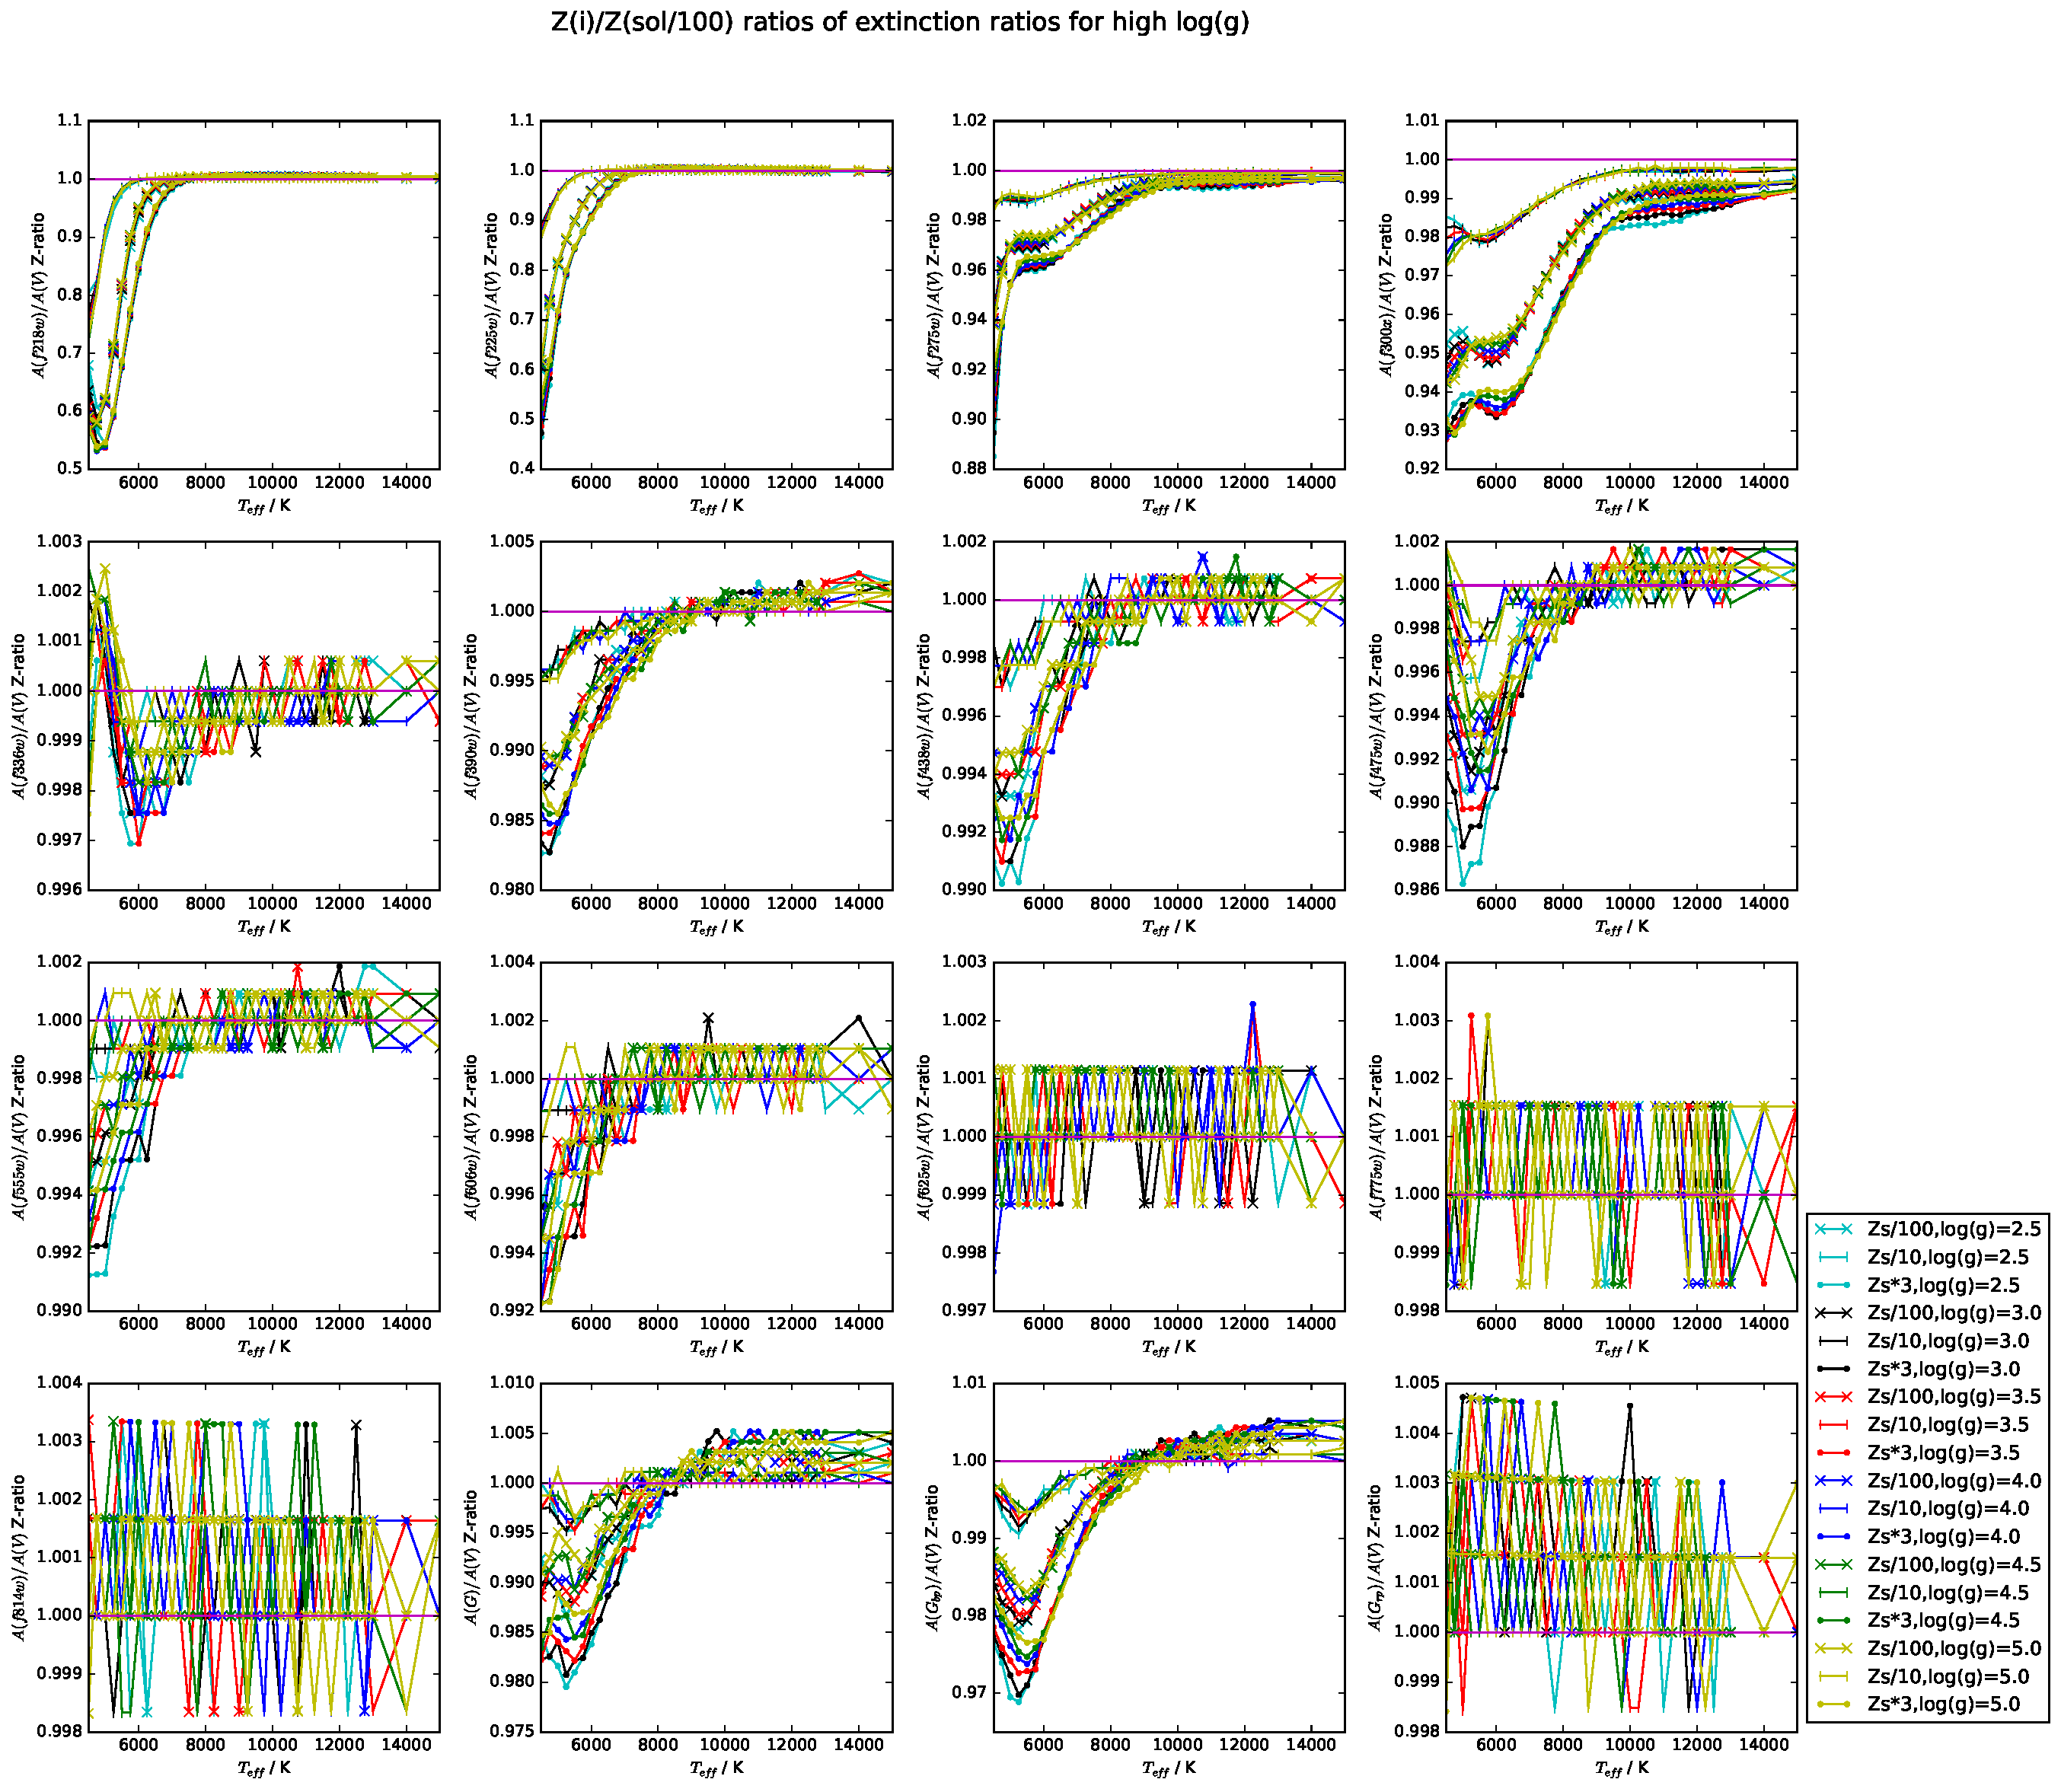
\includegraphics[scale=0.3]{../Aall_ratio_Zs_div_Z2_effect_high_logg_zoom_15000.pdf}
\caption{****psrsoft image output for a simulated pulsar data file}
\label{all_Z_Z2_ratio}
\end{center}
\end{figure}

\begin{figure}
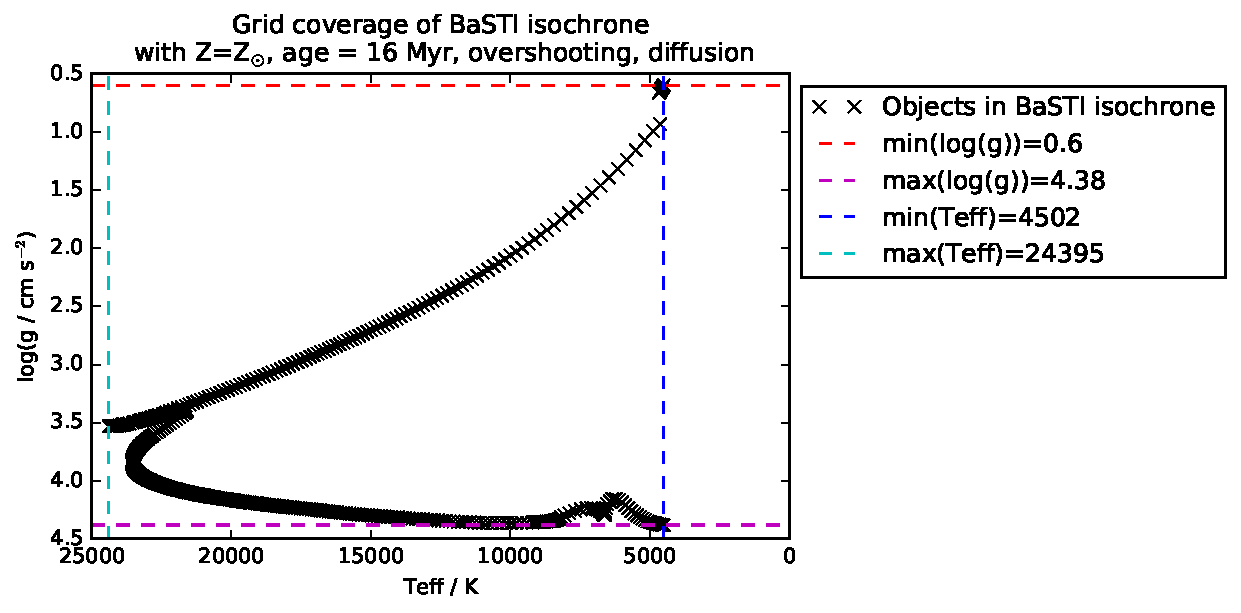
\includegraphics[scale=0.4]{../wfc3_16_23Myr_10Gyr_complex_solar/wfc3_ATLAS9_grid_BaSTI_coverage_c16_complex_Zsol_4500.pdf}
\caption{$T_{\textnormal{eff}}$-log($g$) grid coverage by a 16 Myr, $Z_{\sun}$ BaSTI isochrone ****including mass-loss, core overshooting and }
\label{BaSTI_coverage}
\end{figure}

\begin{figure}
\begin{center}
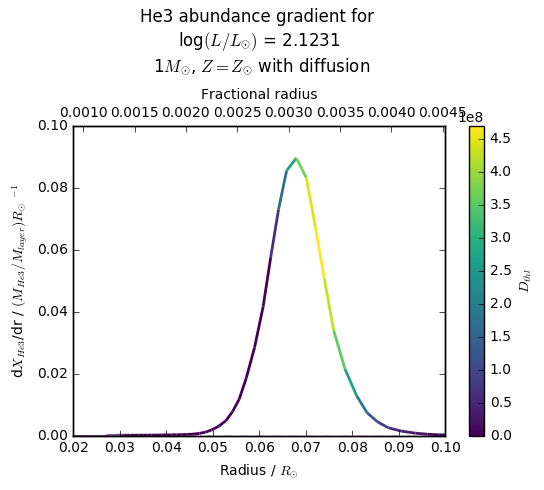
\includegraphics[scale=0.4]{../mu_test_data/mu_test_graphs/eq_logL=2p1231_He3_radius_gradient_Dthl_color.png}
\caption{$^{3}$He abundance gradient for model with $Z = Z_{\sun}$, $M = 1M_{\sun}$ and diffusion effects included, at a point $\log(L/L_{\sun}) = 2.1231$}
\label{dHe3/dr_colour}
\end{center}
\end{figure}

\begin{figure}
\begin{center}
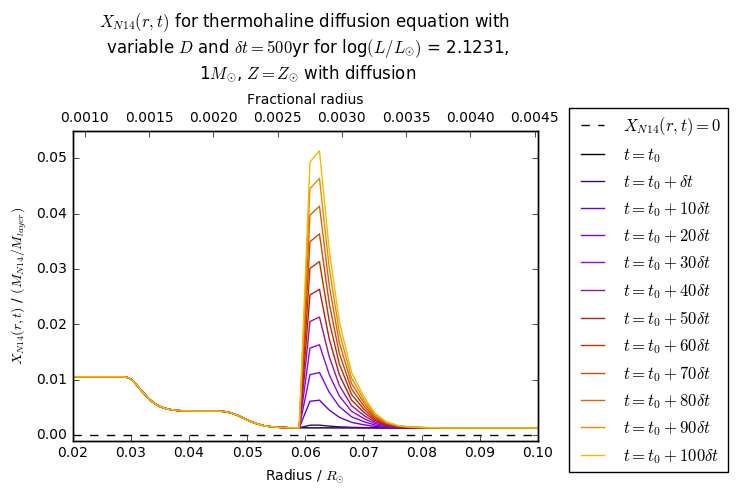
\includegraphics[scale=0.4]{../mu_test_data/mu_test_graphs/eq_logL=2p1231_time_diff_eq_Dvar_10dt_dmu_k_lim.png}
\caption{$^{14}$N abundance time derivative for model with $Z = Z_{\sun}$, $M = 1M_{\sun}$ and diffusion effects included, at a point $\log(L/L_{\sun}) = 2.1231$}
\label{dXN14/dt_colour}
\end{center}
\end{figure}

% ****FORMAT FOR INCLUDING PDF IMAGES!!!
% for guidance, see phd_work/grfguide.pdf
%\includegraphics[<options>]{filename.pdf}


\citet{2017RSOS....470192S}
\citet{2004astro.ph..5087C}
\citet{2004ApJ...612..168P}

\section{Discussion}

\section{Future work}

\bibliographystyle{mnras} % unsrtnat
\bibliography{transfer_report}

\end{document}